\chapter{Demonstrações controladas complementares}\label{ap:demonstracoes}
Os três painéis deste apêndice foram produzidos em um conjunto sintético de 1.000 observações (semente 42), com grupos geradores conhecidos. Eles complementam a leitura dos escores reais do Capítulo~\ref{demonstracao-experimental-das-tecnicas-de-ml}. O ensaio empregou \texttt{RobustScaler} e normalização pelos quantis $P_{01}$--$P_{99}$, segundo a documentação da demonstração. Não se trata da configuração congelada da campanha OOT nem de uma estimativa de acerto de vistorias.

\section{Isolamento global e densidade local}
A Figura~\ref{fig:ml-iforest-microcluster} mostra a projeção dos atributos e a distribuição de escores do Isolation Forest (200 árvores, contaminação de 0,078 no ensaio). O grupo normal possui 922 observações; os demais incluem morfologia rara, outliers locais e globais (20 observações cada) e um microagrupamento de 18. Neste cenário, a mediana normalizada do microagrupamento foi 0,500, abaixo do limiar P95 de 0,564, enquanto a dos outliers globais foi 1,000. O agrupamento compacto pode receber menor pontuação de isolamento mesmo quando suas observações são distintas da população dominante. A projeção bidimensional auxilia a visualização, mas não substitui o espaço de atributos utilizado pelo detector.

\begin{figure}[htbp]\centering\caption{Isolamento global e microagrupamento no experimento controlado}\label{fig:ml-iforest-microcluster}
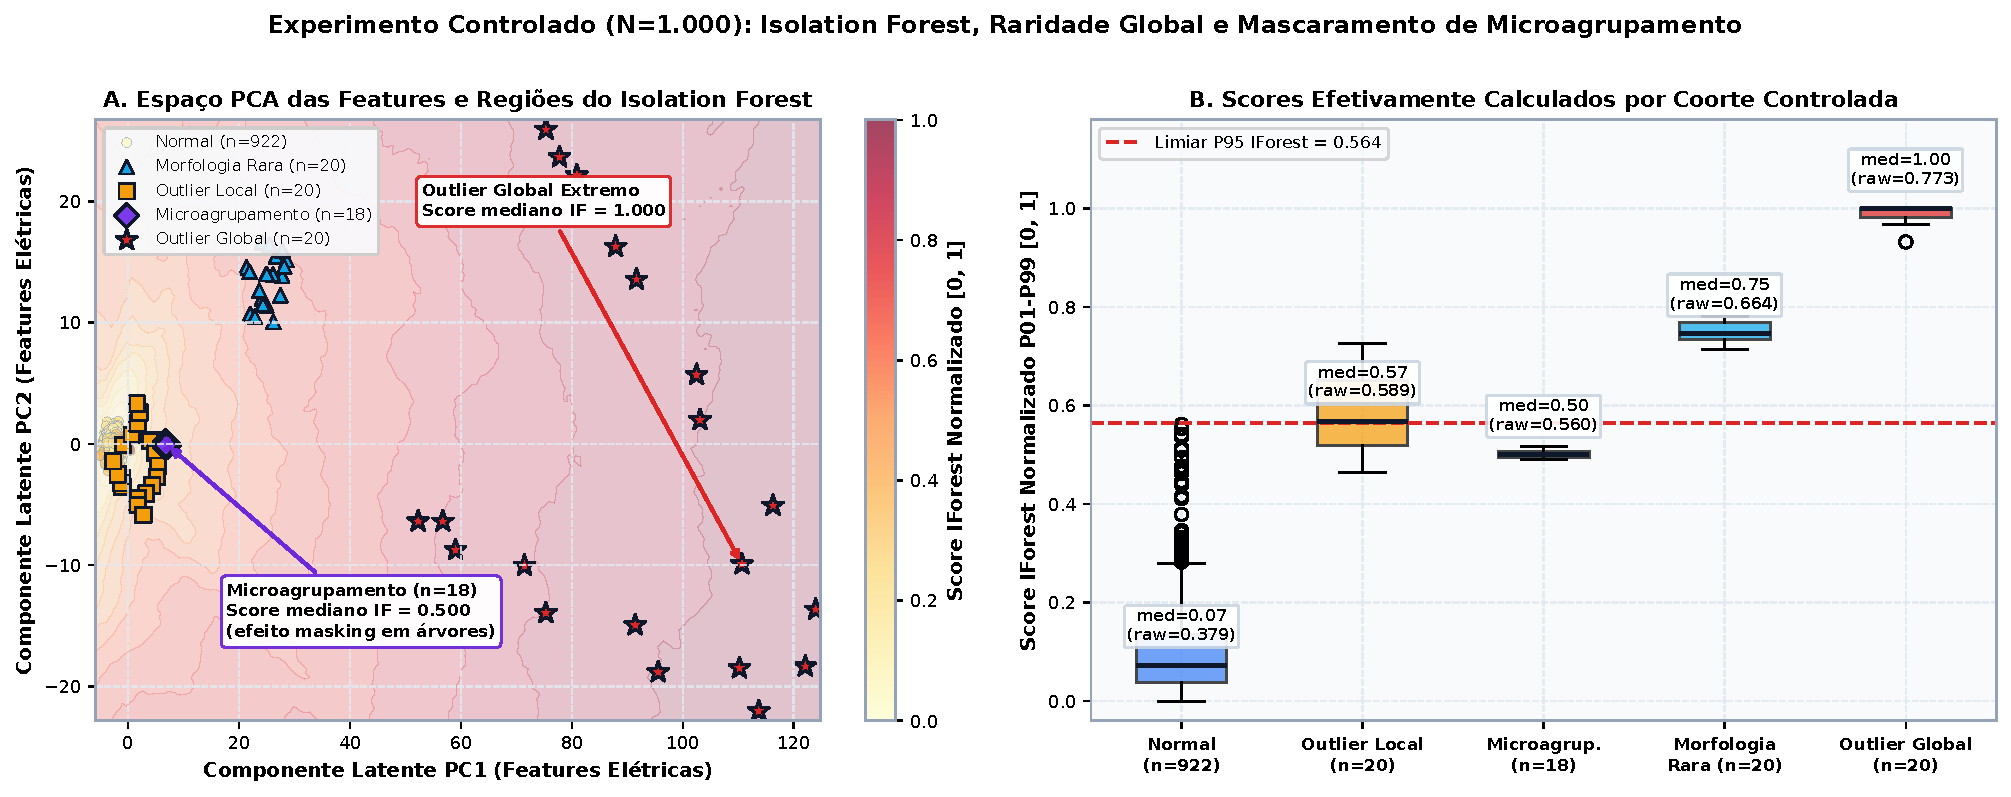
\includegraphics[width=\linewidth,height=0.72\textheight,keepaspectratio]{figuras/fig_5_1a_isolation_forest_microcluster.pdf}
\par\small Fonte: elaboração própria a partir do experimento sintético controlado.
\end{figure}

\clearpage
No LOF (35 vizinhos, número superior ao tamanho do microagrupamento), a comparação de densidades usa uma escala bruta própria, representada em escala logarítmica no painel. Na Figura~\ref{fig:ml-lof-escala-propria}, as medianas de $-\mathrm{NOF}$ (negativo do fator de anomalia retornado pelo detector) são 1,05 no grupo normal, 2,39 no microagrupamento e 3,15 no grupo de outliers locais. Os dois últimos excedem o limiar P95 de 1,99 do ensaio. A divergência frente ao IF ilustra a influência da vizinhança escolhida. Não demonstra que o LOF recupera todos os casos reais omitidos pelo IF; o resultado depende do número de vizinhos, da distribuição e da escala dos atributos.

\begin{figure}[htbp]\centering\caption{Escalas bruta e normalizada do LOF e comparação com o IF no ensaio controlado}\label{fig:ml-lof-escala-propria}
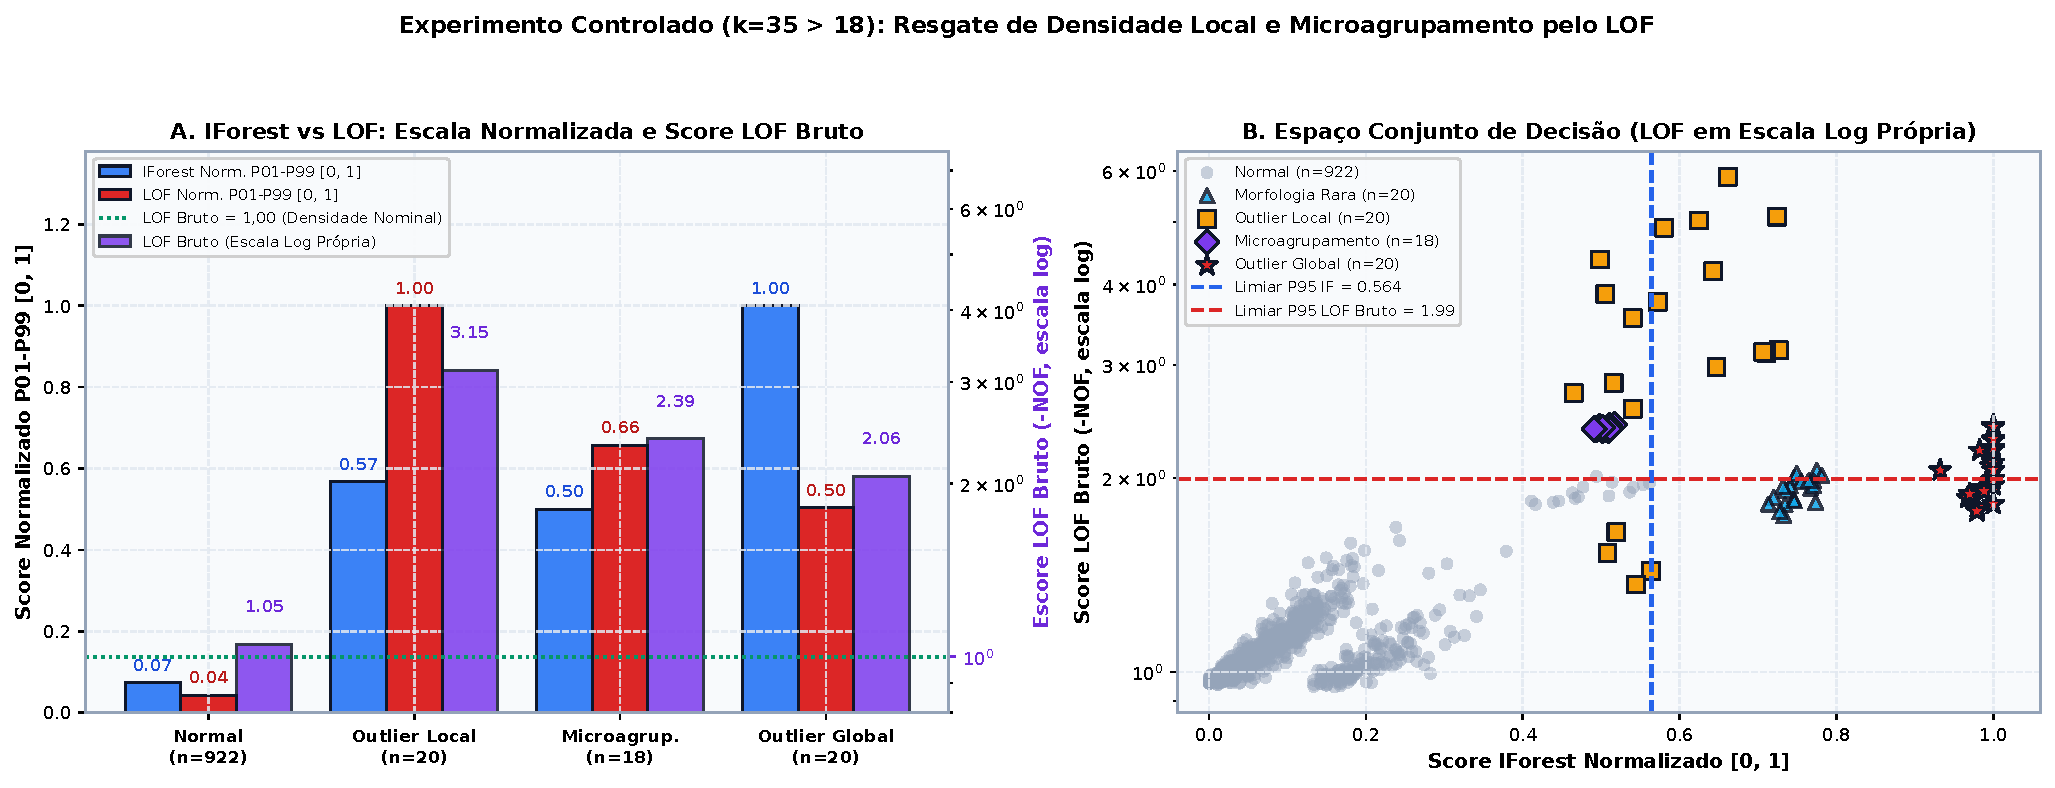
\includegraphics[width=\linewidth,height=0.72\textheight,keepaspectratio]{figuras/fig_5_1b_lof_escala_propria.pdf}
\par\small Fonte: elaboração própria a partir do experimento sintético controlado.
\end{figure}

\clearpage
\section{Contextualização por circuito}
A Figura~\ref{fig:ml-contextualizacao-percentis} compara percentis empíricos globais e locais nos quatro circuitos simulados. As posições acima e abaixo da diagonal representam, respectivamente, promoção e atenuação no contexto local. No corte percentílico de 95\%, registraram-se sete promoções e seis atenuações, com Jaccard de 0,776 reportado no painel para o Top-5\%. As cardinalidades podem diferir com o uso de limiar percentílico e empates. As diferenças ilustram a mudança de referência estatística quando se compara uma observação com os pares do próprio circuito. Não constituem prova de maior precisão da seleção no parque real.

\begin{figure}[htbp]\centering\caption{Comparação entre percentis globais e locais em quatro circuitos simulados}\label{fig:ml-contextualizacao-percentis}
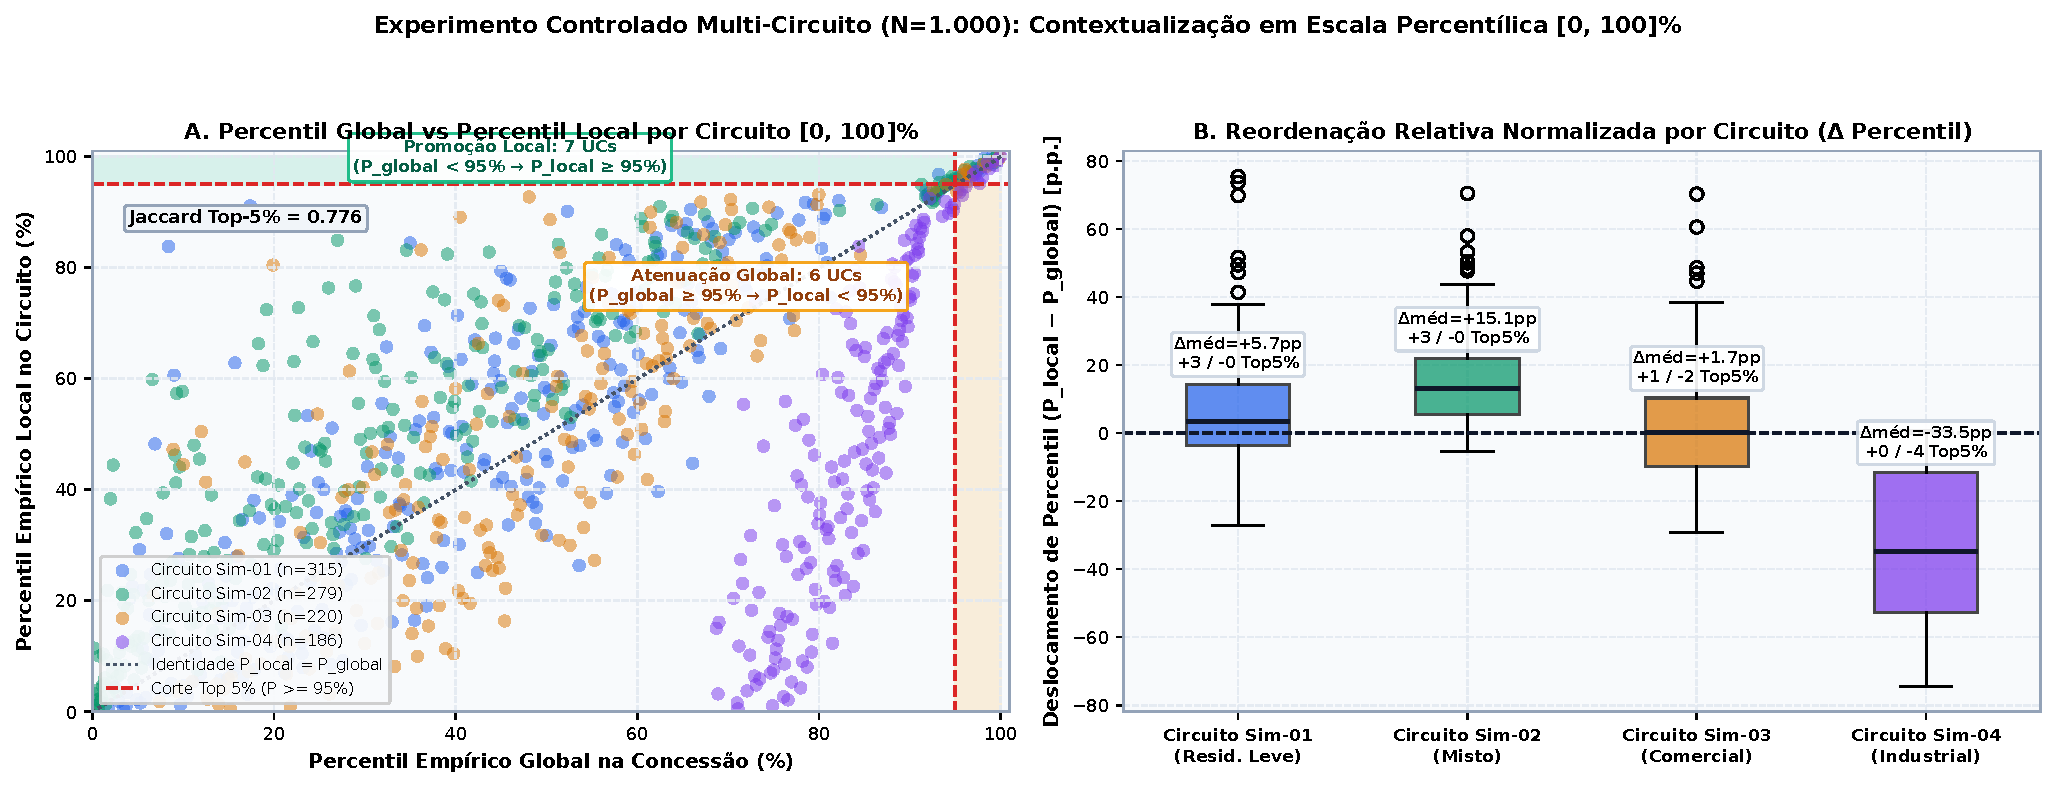
\includegraphics[width=\linewidth,height=0.72\textheight,keepaspectratio]{figuras/fig_5_1c_contextualizacao_percentis.pdf}
\par\small Fonte: elaboração própria a partir do experimento sintético controlado.
\end{figure}
